\section{iClusterVB methodology and practical steps}

\subsection{iClusterVB methodology}

The \texttt{iClusterVB} framework is built on a Bayesian model-based clustering approach using a finite mixture model, variational inference, and embedded feature selection.

\subsection{Finite Mixture Model}

A finite mixture model is a probabilistic model that represents a population as a mixture of 
several subpopulations, each described by its own probability distribution. 
It is widely used in clustering and density estimation. 
\footnote{For more details, refer 
to the \href{https://en.wikipedia.org/wiki/Mixture_model}{Wikipedia article on finite mixture models}.}

Let $\mathbf{x}_i = (x_{i1}, \ldots, x_{ip})^\top$ be the $p$-dimensional 

feature vector for individual $i$, and let $z_i$ be the cluster assignment. 
The likelihood of the data is modeled using a finite mixture model:
\[
P(\mathbf{x}_i \mid \boldsymbol{\pi}, \Theta) = \sum_{k=1}^{K} \pi_k P(\mathbf{x}_i \mid \phi_k)
\]

Assuming conditional independence of features within each cluster:

\[
P(\mathbf{x}_i \mid \phi_k) = \prod_{j=1}^{p} P(x_{ij} \mid \phi_{kj})
\]

where $\phi_k$ are parameters for the $k$-th cluster, and $\pi_k$ are mixing proportions such that $\sum_k \pi_k = 1$.

\subsection{Feature Selection}

To select informative features, the model includes a latent indicator $\gamma_{ij} \in \{0,1\}$ that controls whether feature $j$ is relevant for clustering:

\[
P(x_{ij} \mid \gamma_{ij}, z_i = k) = 
\begin{cases}
P(x_{ij} \mid \theta_{kj}), & \text{if } \gamma_{ij} = 1 \\
P(x_{ij} \mid \eta_j), & \text{if } \gamma_{ij} = 0
\end{cases}
\]

The marginal likelihood becomes:

\[
P(\mathbf{x}_i \mid z_i = k) = \prod_{j=1}^{p} \left[ \omega_j P(x_{ij} \mid \theta_{kj}) + (1 - \omega_j) P(x_{ij} \mid \eta_j) \right]
\]

where $\omega_j$ is the inclusion probability of feature $j$.

\subsection{Prior Distributions}

Priors are imposed to enable Bayesian inference, leveraging the conjugate prior method for computational efficiency and analytical tractability. Conjugate priors ensure that the posterior distribution belongs to the same family as the prior, simplifying updates during inference.

\begin{table}[h!]
\centering
\begin{tabular}{|c|c|c|c|}
\hline
\textbf{Likelihood Function} & \textbf{Parameter} & \textbf{Prior Distribution} & \textbf{Posterior Distribution} \\ \hline
$P(\mathbf{x}_i \mid \boldsymbol{\pi})$ & $\boldsymbol{\pi}$ & Dirichlet$(\alpha_0)$ & Dirichlet$(\alpha_0 + \text{counts})$ \\ \hline
$P(x_{ij} \mid \mu_{kj}, \sigma^2_{kj})$ & $\mu_{kj}$ & $\mathcal{N}(\mu_0, s_0^2)$ & $\mathcal{N}(\mu_n, s_n^2)$ \\ \hline
$P(x_{ij} \mid \sigma^2_{kj})$ & $\sigma^2_{kj}$ & $\text{IG}(a_0, b_0)$ & $\text{IG}(a_n, b_n)$ \\ \hline
$P(x_{ij} \mid \boldsymbol{\theta}_{kj})$ & $\boldsymbol{\theta}_{kj}$ & Dirichlet$(\boldsymbol{\kappa}_{kj})$ & Dirichlet$(\boldsymbol{\kappa}_{kj} + \text{counts})$ \\ \hline
$P(x_{ij} \mid \lambda_{kj})$ & $\lambda_{kj}$ & Gamma$(c_0, d_0)$ & Gamma$(c_n, d_n)$ \\ \hline
\end{tabular}
\caption{Conjugate Priors and Corresponding Posterior Distributions with Likelihood Functions and Parameters}
\label{tab:conjugate_priors}
\end{table}

\begin{itemize}
  \item \textbf{Mixing weights:} $\boldsymbol{\pi} \sim \text{Dirichlet}(\alpha_0)$ ensures that the mixing proportions are non-negative and sum to 1. The posterior updates naturally with observed cluster counts.
  \item \textbf{Gaussian features:} Conjugate priors for mean ($\mathcal{N}$) and variance ($\text{IG}$) allow efficient updates based on sufficient statistics (e.g., sample mean and variance).
  \item \textbf{Categorical features:} Dirichlet priors for multinomial parameters $\boldsymbol{\theta}_{kj}$ simplify posterior updates with observed category counts.
  \item \textbf{Count features:} Gamma priors for Poisson rates $\lambda_{kj}$ provide a flexible framework for modeling count data, with posterior updates driven by observed counts.
\end{itemize}

\subsection{Variational Inference}

  To approximate the posterior distribution $P(\beta \mid \mathbf{X})$, iClusterVB uses a method called variational inference. 
  Instead of relying on computationally expensive sampling methods, it turns the problem into an optimization task.

  The goal is to find a simpler distribution $Q(\beta)$ that is as close as possible to the true posterior
  $P(\beta \mid \mathbf{X})$. This is done by minimizing a measure called KL divergence,
  which quantifies the difference between the two distributions:

  \[
  \text{KL}(Q(\beta) \parallel P(\beta \mid \mathbf{X})) = \int Q(\beta) \log \frac{Q(\beta)}{P(\beta \mid \mathbf{X})} \, d\beta
  \]

  In practice, this is equivalent to maximizing a quantity called the Evidence Lower Bound (ELBO). The ELBO is defined as:

  \[
  \text{ELBO} = \mathbb{E}_{Q(\beta)}[\log P(\mathbf{X}, \beta)] - \mathbb{E}_{Q(\beta)}[\log Q(\beta)]
  \]

  The ELBO balances two terms: how well the model explains the data and how simple the approximating distribution is.

  Additionally, iClusterVB can automatically adjust the number of clusters by checking the estimated 
  mixing proportions $\hat{\pi}_k$. If a cluster's proportion is too small (e.g., below a threshold like 0.01),
  that cluster is removed to simplify the model.

\subsection{Practical Steps of implementing iClusterVB}

\begin{description}
  \item[Step 1: Finite Mixture Model] 
  The first step is using a finite mixture model which assumes the data arises from hidden clusters. Each cluster has its own distribution, and a latent variable determines group membership.

  \item[Step 2: Feature Selection] 
  iClusterVB performs feature selection by assigning a probability to each feature, indicating its relevance. Irrelevant features are dropped, improving interpretability.

  \item[Step 3: Prior Distributions] 
  Cluster proportions are given a Dirichlet prior. Relevant features get conjugate priors (normal/inverse gamma), while irrelevant features are estimated via MLE.

  \item[Step 4: Variational Inference] 
  Variational Bayes transforms the inference problem into an optimization task, maximizing the Evidence Lower Bound (ELBO) for faster convergence compared to MCMC.

  \item[Step 5: Model Selection] 
  The number of clusters is selected based on model fit criteria, ensuring robustness and reliability.
\end{description}

\textcolor{red}{put the code here or in the appendix}

\begin{figure}[!h]
\centering
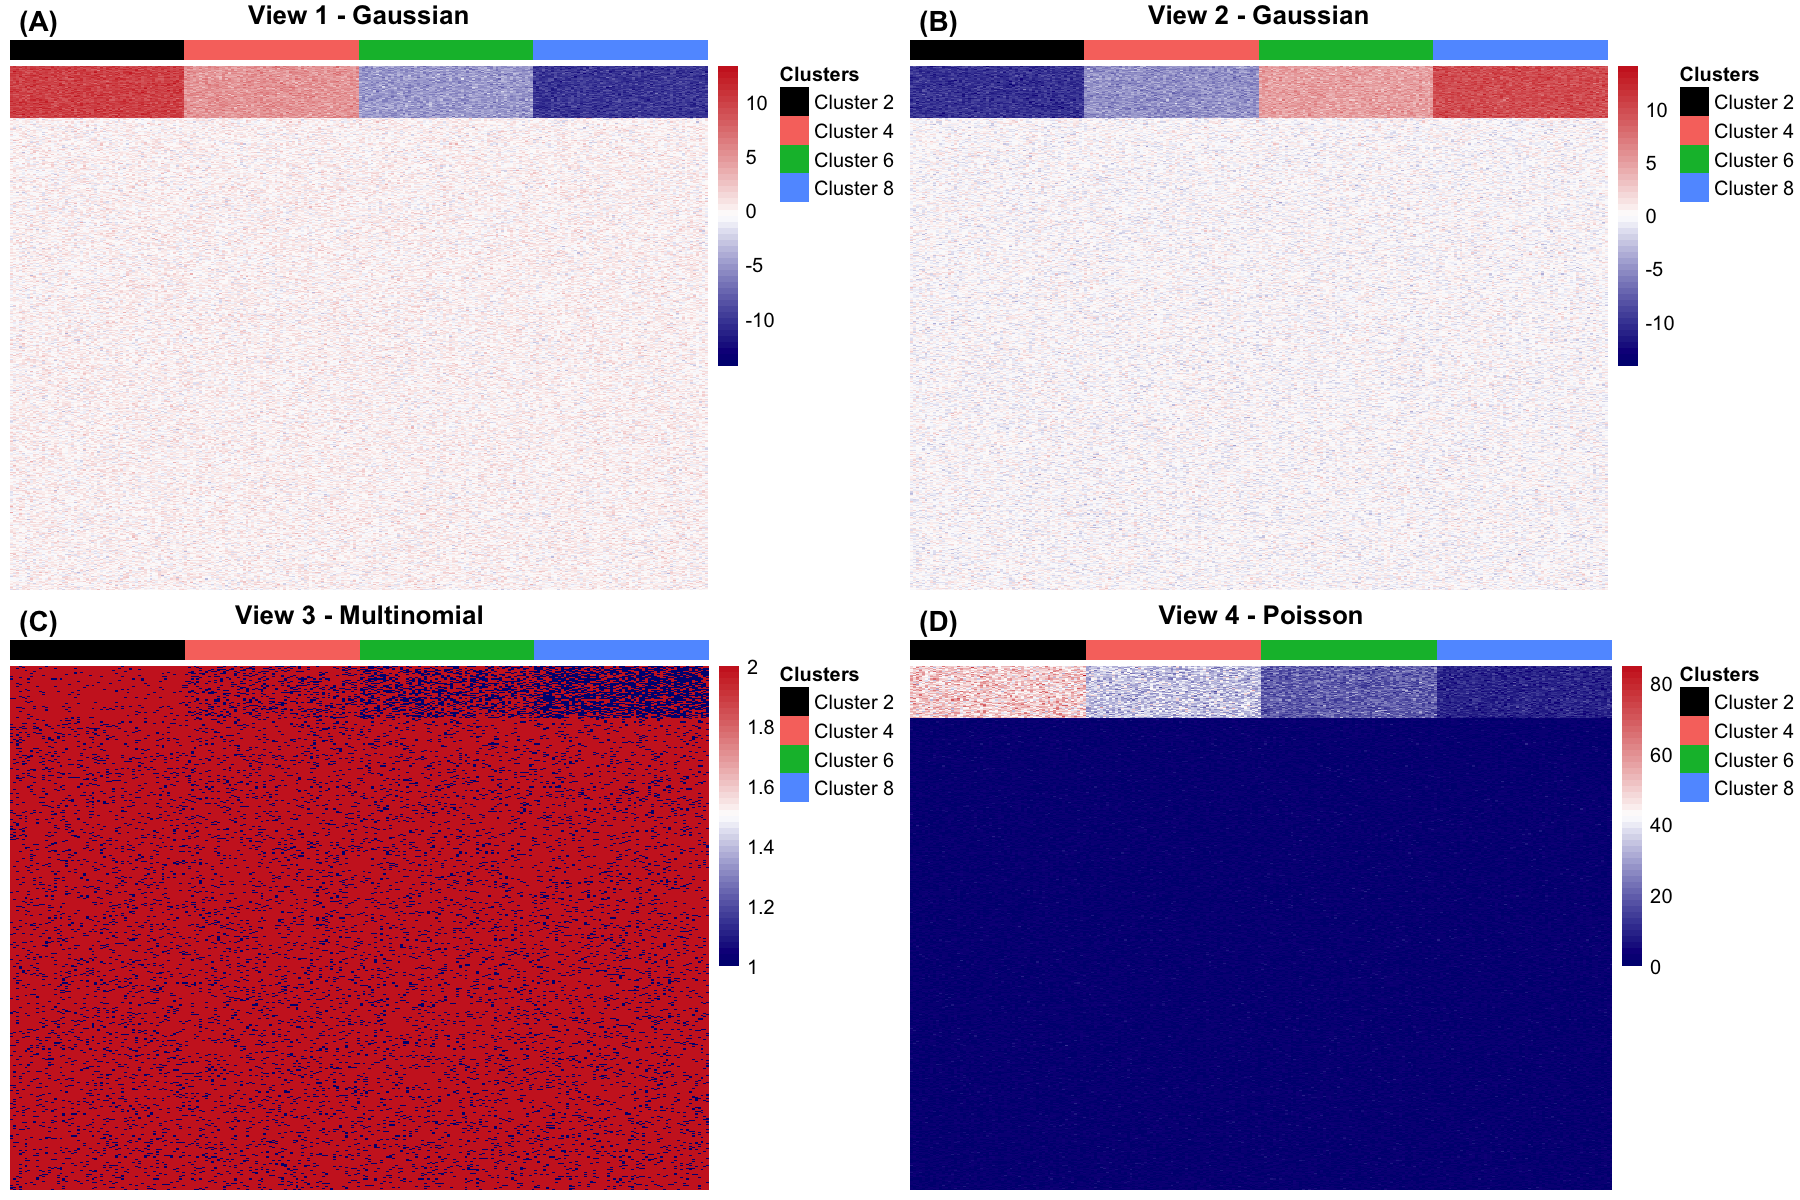
\includegraphics[width=0.9\textwidth]{../results/Simulated_heatmap.png}
\caption{Heat map of simulated data with 4 clusters}
\label{fig:simulated_heatmap}
\end{figure}